% !TeX root = ../../../thesis.tex

\subsection{Pseudorandom Noise Sequences}
\label{subsec:pn-sequences}

PN sequences are sequences which look like they are randomly generated but they are easily generated in software or hardware.
They are generated with linear shift registers of length $n$.
The sequences have the following noise-like properties~\cite{mitra2008pseudo}:

\begin{itemize}
	\item Balance property:	Any PN sequence of length $L = 2^n - 1$ contains exactly $2^{n-1}$ ones and exactly $2^{n-1} - 1$ zeros.

	\item Runs property: A run is a subset of the sequence where all the consecutive numbers are the same. In any PN sequence, $1/2$ of the runs have length 1, $1/4$ have length 2, $1/8$ have length 3 and so on.

	\item Auto-correlation property: The auto-correlation function of a PN sequence will take on two values as can be seen in \autoref{eq:autocorr-pn} and \autoref{fig:autocorr-pn}.


\end{itemize}






\begin{equation}
	\label{eq:autocorr-pn}
	R(\tau) = 
		\begin{cases}
			L    & \quad \text{if } \tau = 0 \\
			-1   & \quad \text{if } \tau \neq 0 \\
		\end{cases}
\end{equation}






\begin{figure}[t]
	\centering
	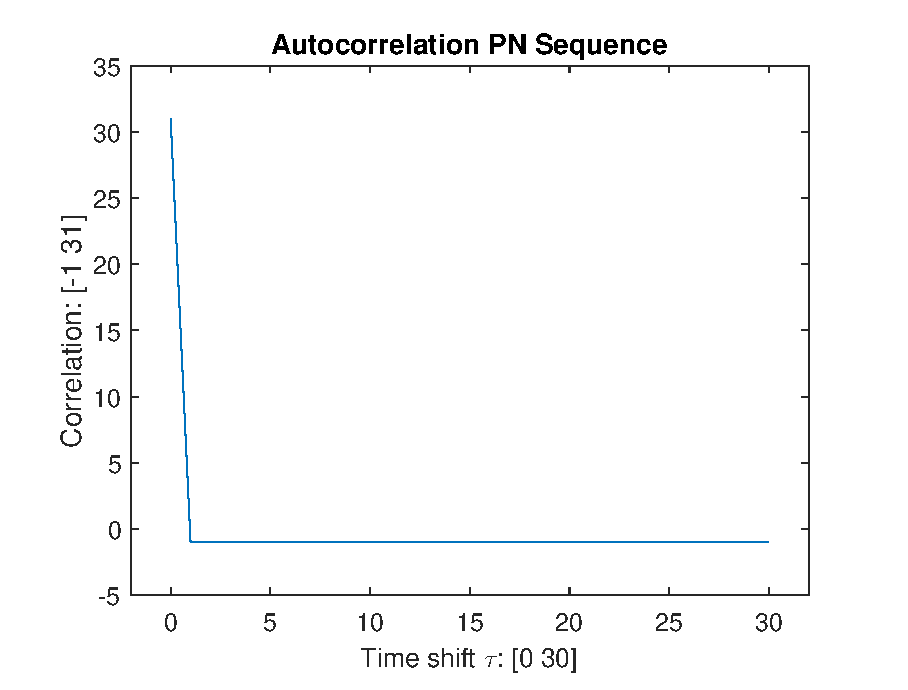
\includegraphics[width=\textwidth]{chapters/cdma-chapters/codes/autocorr-pn.eps}
	\caption{Autocorrelation of PN sequence of length 31.}
	\label{fig:autocorr-pn}
\end{figure}





PN sequences are generated using a linear feedback shift register (LFSR) \cite{Wang:1988:LFS:52007.52024}.
\autoref{fig:lfsr} shows an $n$ length LFSR with XOR gates attached to it.
The LFSR is defined entirely by the feedback function, also called a characteristic polynomial.
It determines the length and the type of sequence generated.
The polynomial looks like \autoref{eq:lfsr-polynomial}.

\begin{equation}
	\label{eq:lfsr-polynomial}
	p(x) = x^n + C_{n-1} x^{n-1}  + C_{n-2} x^{n-2} + \dotsc + C_{2} x^{2}  + C_{1} x  + C_{0}
\end{equation}

\begin{figure}[t]
	\centering
	\begin{tikzpicture}


		\node[block                  ] (last_register) {$s_{n-1}$};
		\node[block, right = 1cm of last_register] (second_last_register) {$s_{n-2}$};
		\draw[line] (last_register.east) -- (second_last_register.west) ;

		\node[block, right = 3cm of second_last_register] (second_register) {$s_{1}$};
		\node[block, right = 1cm of second_register] (mid_register) {$s_{0}$};
		\draw[line] (second_register.east) -- (mid_register.west) ;

		\draw[dashed, line] (second_last_register.east) -- (second_register.west) ;

		\node[coordinate, right = 2cm of mid_register] (output_point) {};
		\draw[line] (mid_register.east) -- (output_point.west) node [midway, above] {output};

		\node[XOR, scale=2, below = 2cm of second_register] (first_xor) {};
		\draw[line] (second_register.south) -- (first_xor.north) node [midway, right] {$C_1$};
		\draw[line] (mid_register.south) |- (first_xor.east) node [pos=0.21, right] {$C_0$};

		\node[coordinate, right = 1.5cm of second_last_register] (h) {};
		\node[XOR, scale=2, below = 2.5cm of h] (mid_xor) {};
		\draw[line] (first_xor.west) -- (mid_xor.east) ;
		\draw[dashed, line] (h.south) -- (mid_xor.north) ;

		\node[XOR, scale=2, below = 2cm of second_last_register] (second_last_xor) {};
		\node[XOR, scale=2, below = 2cm of last_register] (last_xor) {};

		\draw[line] (second_last_register.south) -- (second_last_xor.north) node [midway, right] {$C_{n-2}$};
		\draw[line] (mid_xor.west) -- (second_last_xor.east) ;
		
		\draw[line] (second_last_xor.west) -- (last_xor.east) ;
		\draw[line] (last_register.south) -- (last_xor.north) node [midway, right] {$C_{n-1}$};

		\node[coordinate, left = 1cm of last_register] (return_point) {};
		
		\draw[line] (last_xor.west) -| (return_point) -- (last_register.west) ;




	\end{tikzpicture}
	\caption{Linear feedback shifter register of length $n$, with XOR gates, to produce a PN sequence.}
	\label{fig:lfsr}
\end{figure}


For PN sequences, there exists no formula for the cross-correlation of two different PN sequences. 
Exhaustive analysis is required to find out which sequences or entire sets have the cross-correlation characteristics that are good enough for the user's application.
In \autoref{tbl:pn-sequences-C-and-cross-corr} the calculated peak cross-correlations per PN sequences in the same set can be found.



The size of the code set is limited.
For a LFSR with $n$ registers, the maximum number of possible codes $C$ is given by \autoref{eq:num-of-pn-codes} \cite{mutagi1996pseudo}, where $P_i$ are the prime factors of $2^n - 1$ and $\alpha_i$ is the power of $i$th prime factor.

\begin{equation}
	\label{eq:num-of-pn-codes}
	C = \frac{1}{n} \prod \{ P_{i} ^ {(\alpha_i - 1)} \times (P_i - 1) \}
\end{equation}

For example when using a LFSR of size $n = 6$, $2^n - 1 = 63$, which can be factored into $3^2 \times 7$.
Giving $P_1 = 3$, $P_2 = 7$, $\alpha_1 = 2$ and $\alpha_2 = 1$.
Thus, the maximum number of codes is: $C = \frac{1}{6} \times \{ 3^{2 - 1} \times (3 - 1) \} \times \{ 7^{1 - 1} \times (7 - 1) \} = 6$.
Another example: Say there are going to be 144 user, so 144 codes are needed. 
This means a code length of 4095 chips.
For PN sequences of other lengths, see \autoref{tbl:pn-sequences-C-and-cross-corr} for the number of codes.


\begin{table}[tbp]
	\centering
	\begin{tabular}{  | l | l | l | }

		\hline
		Code Length (L)	& Number of Codes (C) 	& Peak cross-correlation	\\ \hline
		
		7				& 2						& 5						\\ \hline					
		15				& 2						& 9						\\ \hline			
		31				& 6						& 11					\\ \hline			
		63				& 6						& 23					\\ \hline		
		127				& 18					& 41					\\ \hline		
		255				& 16					& 95					\\ \hline	
		511				& 48					& 113					\\ \hline	
		1023			& 60					& 383					\\ \hline		
		2047			& 176 					& 287					\\ \hline		
		4095			& 144					& 144					\\ \hline		


	\end{tabular}
	\caption{Table showing the number of PN sequences of the same length along with the peak cross-correlation \cite{kettunen1997code}. }
	\label{tbl:pn-sequences-C-and-cross-corr}

\end{table}


To conclude: PN sequences have less number of sequences in the same set, compared to orthogonal sequences.
But the auto- and cross-correlation are better than those of the orthogonal sequences.
And these auto- and cross-correlation numbers also hold when the sequences are sent asynchronously.










